\chapter{Operation of the \abbrROV} \label{app:operation}
This Chapter describes normal operation of the \abbrROV, how to implement new controllers and some tips for troubleshooting.
 
\section{Start up of the \abbrROV}
For starting the \abbrROV connect all cables according to \Sectionref{sec:wiring}.
\begin{itemize}
	\item Make sure that the battery is tightly fastened and is fully charged. 
	\item Slide the cradle gently into the \abbrROV tube. 
	\item If needed apply some silicone grease to the O-rings of the end cap. Then slide the end cap into the \abbrROV tube.
	\item Insert the vent bolt in to the vent nut on the end cap.
	\item Insert the cat 6 cable to the workstation.
 \end{itemize} 
Navigate to the catkin\_ws folder on the workstation and run the start script in a terminal for the \abbrROV
\begin{lstlisting}
 ./startrov.sh
\end{lstlisting}
Then in a new terminal navigate to the catkin\_ws folder and run the workstation script
\begin{lstlisting}
 ./startworkstation.sh
\end{lstlisting} 
%%%%%%%%%%%%%%%%%%%%%%%%%%%%%%%%%%%%%%%%%%%%%%%%
\section{Operating the ROV}

\subsection{Modes and controllers}

\subsubsection{Manual mode}

\subsection{Logging data}\label{sec:logging}
For logging data rqt-bag or the supplied script can be used. In rqt on the workstation start rqt-bag by Plugins $\rightarrow$ Logging $\rightarrow$ Bag. Start the recording of data by pressing the red circle. A menu of available topics is showed, select the topics that you want to record. Then give the logfile a name in the pop-up.
To stop recording data press the red circle and close Bag by Running $\rightarrow$ Close:Bag. For using the logging scripts use 
\begin{lstlisting}
./test.sh
\end{lstlisting}
and follow the instructions.

\subsection{Sending test signals}
For sending telegraph signals to the \abbrROV the logging script in \Sectionref{sec:logging} can be used or dynamic reconfigure can be used. Dynamic reconfigure can be used from the command line or rqt. In rqt start dynamic reconfigure by Plugins $\rightarrow$ Configuration $\rightarrow$ Dynamic Reconfigure. When the dynamic reconfigure box is shown choose matlab\_controller then check telegraph\_signals. In the submenu choose the scaling and switch factor for each thruster.
To enable tests change the test signal from off $\rightarrow$ on.    

\subsection{Displaying the continuous plots}
Displaying plots in rqt is enabled by Plugins $\rightarrow$ Visualization $\rightarrow$ Plot. In the plot plugin plot data by choosing topics in the topic field. The active topics can be seen in the command line by running 
\begin{lstlisting}
rostopic list
\end{lstlisting}
For multiarray messages an extra \textit{\textbackslash data} field has to be added to the topic. Data is then accessed by indexing with hard brackets. 
\begin{example}
Plot the data with index 0 in the multiarray message on topics \textit{/rovio/imu/data}. Type /rovio/imu/data/data[0] in the into the topic field and press the green plus.  
\end{example}

\subsection{\abbrLED lights on the HKPilot}
There are several different \abbrLED lights on the HKPilot Mega 2.7, \Tableref{tab:ledStatus} summaries some of \abbrLED statuses
 \begin{table}[tbp]
  \centering
  \caption{\label{tab:ledStatus}%
    Some of the \abbrLED statues used by the HKPilot Mega 2.7.}
  \begin{tabular}{l p{0.7\linewidth}}
    \toprule%
    \textbf{Light}  & \textbf{Description} \\
    \otoprule%
    Red 				& The HKPilot is setting up sensors and a connection to \abbrROS. The red light won't turn off until the connection to \abbrROS has been established.\\
    \midrule
    Pulsating blue 	& Pulsating blue light indicate that the HKPilot has connection with the workstation.\\
    \midrule
    Yellow 			& Shows that the \abbrROV is disarmed. \\
    \bottomrule%
  \end{tabular}
\end{table}

%%%%%%%%%%%%%%%%%%%%%%%%%%%%%%%%%%%%%%%%%%%%%%%%
\section{New Parameter Estimation and New Controllers}

\subsection{New Controllers}
To implement a new controller open the Simulink file Controller.slx. 


\begin{tikzpicture}
    \node[anchor=south west,inner sep=0] (image) at (0,0) {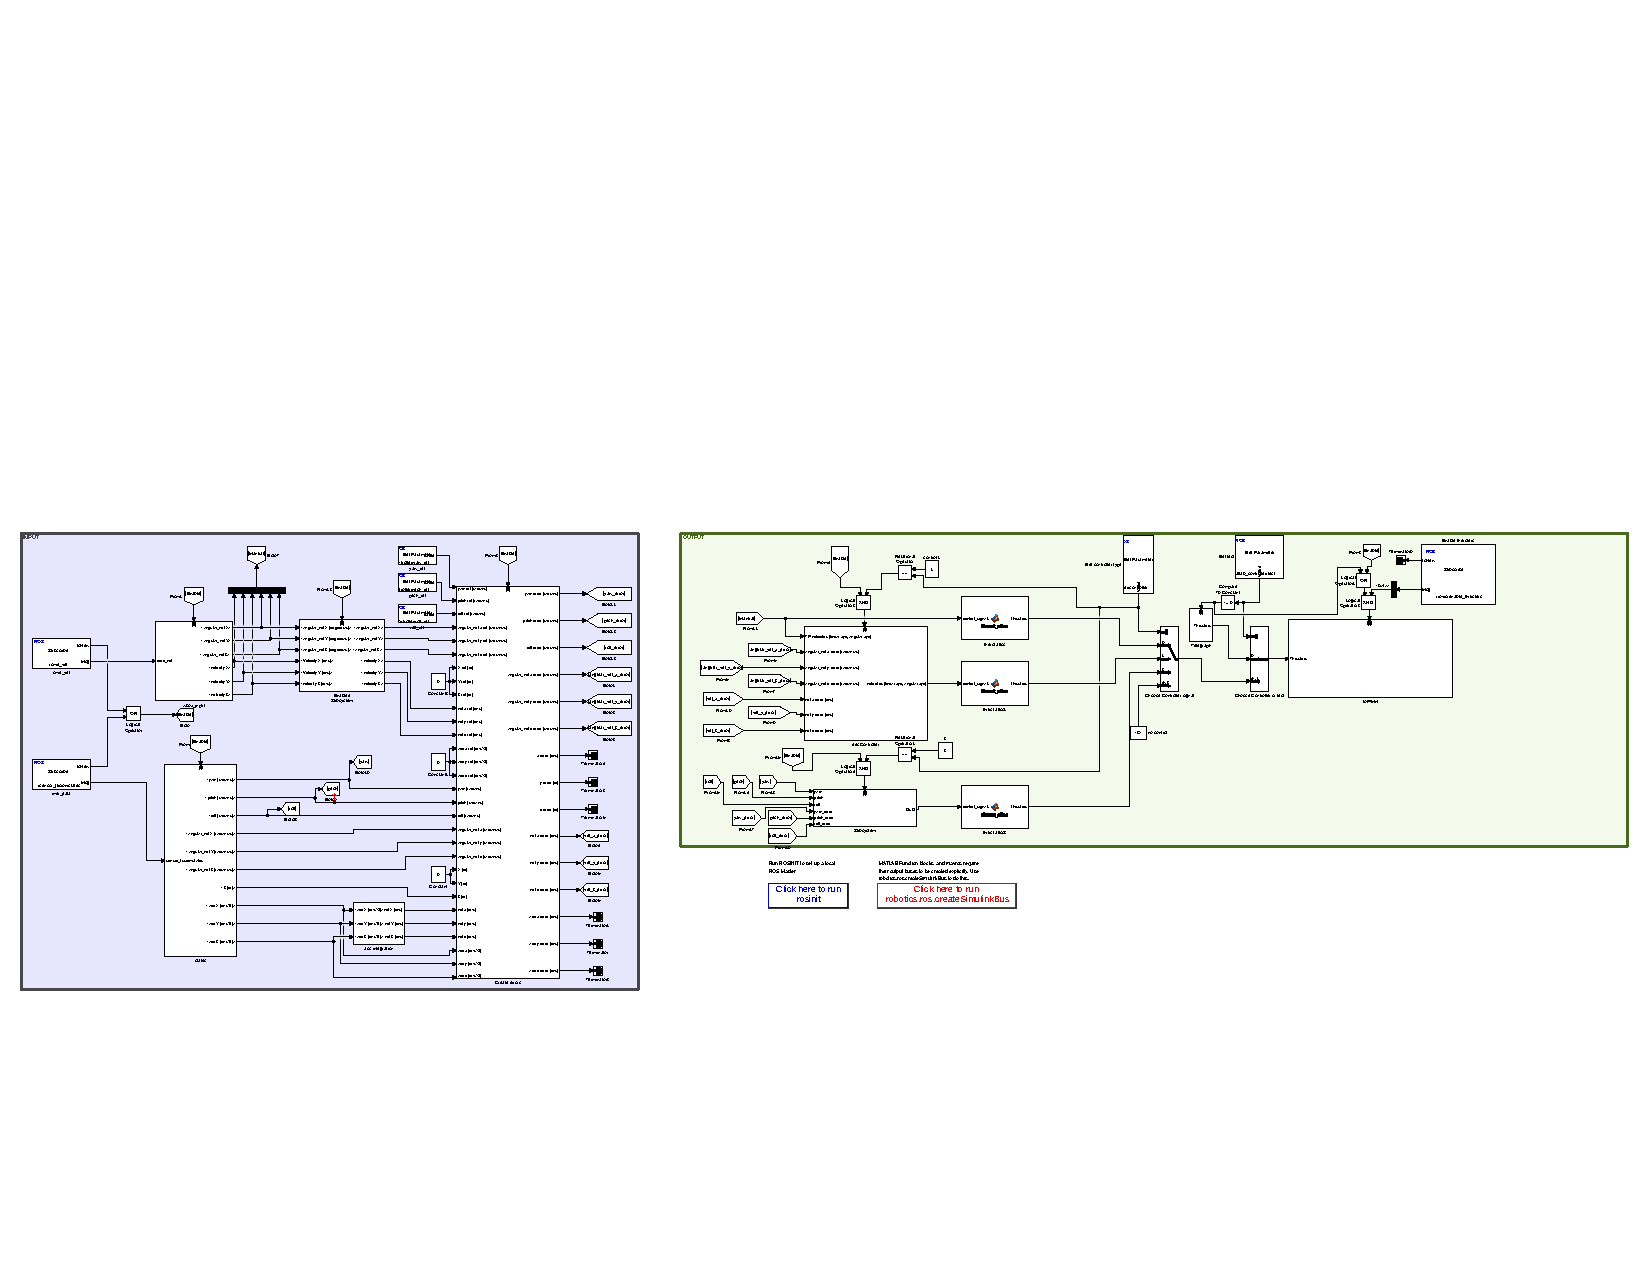
\includegraphics[trim={18cm 7cm 2.5cm 9cm},clip,width=0.9\textwidth]{Controller}};
    \begin{scope}[x={(image.south east)},y={(image.north west)}]
        \draw[red,ultra thick,rounded corners] (0.62,0.65) rectangle (0.78,0.75);
    \end{scope}
    \caption{}
    \label{fig:Controller}
\end{tikzpicture}

\subsection{New Parameter Estimation}

\subsection{Code Generation of the Controller Node}


%%%%%%%%%%%%%%%%%%%%%%%%%%%%%%%%%%%%%%%%%%%%%%%%
\section{Known issues and troubleshooting}

\subsection{\abbrROS debugging}

\subsection{Check Ethernet connection}
It is assumed that the setup from \Appref{app:dependencies} is done. To check the Ethernet connection from the \abbrROV to the workstation or the other way around do
\begin{lstlisting}
#From the ROV to the workstation
ping -c 10 10.0.0.10 
#From the workstation to the ROV
ping -c 10 10.0.0.20
\end{lstlisting}
If the connection is good the output ought to be something like 64 bytes received from 10.0.0.10... Otherwise the connection has to be checked. Check that the Ethernet cable is connected and that both the \abbrROV and workstation is powered on. Check that both the workstation and the \abbrROV has the correct \abbrIP by the command
\begin{lstlisting}
ifconfig
\end{lstlisting}
The output at eth0 ought to contain the correct \abbrIP. Otherwise the setup from the \Appref{app:dependencies} has to revisited.

\subsection{One or several thrusters are unresponsive}
To check for unresponsive thrusters run the following commands 
\begin{lstlisting}
rostopic pub --once /rovio/thrusters_enable std_msgs/Bool true
./thrusterTest.sh
\end{lstlisting}
The thruster test will run the thrusters at a minimal torque in incremental order. If the one or several thrusters are unresponsive check that the thrusters are connected according to \Sectionref{sec:wiring}. If all thrusters are unresponsive check that the HKPilot Mega 2.7 and the Raspberry has power and connected to each other. 

\subsection{Checking and changing polarity of thrusters}
